\chapter{Revisão Teórica}
\label{cap:rev.teorica}
\thispagestyle{plain}
\graphicspath{{./Cap2_Revisao_Teorica/Figures/}}

\section{O problema da segurança em espaços públicos e privados}
O problema de segurança pública no Brasil é algo que está sempre em evidência. O Programa das Nações Unidas para o Desenvolvimento (Pnud), em seu relatório divulgado em 12/11/2013, constata que o Brasil apresentou a maior taxa de roubo da América Latina, segundo dados de 2011 repassados pelos países. Os dados apontam que para cada 100 mil habitantes no Brasil, há 572,7 ocorrências de roubo. E sabe-se que, na realidade, esse número tende a ser maior, tendo em vista que nem todos os roubos são reportados às autoridades \cite{G12013}.

Estima-se um total de 15 milhões de ocorrências de roubos e furtos no Brasil no ano de 2003, incluído os casos que não foram notificados. E como parte da consequência, estima-se uma perda material de R\$ 8,4 bilhões \cite{Cerqueira2007}. Se corrigido para o ano de 2020 com base no IPCA (Índice de Preços ao Consumidor Amplo), esse valor seria de aproximadamente R\$ 20,2 bilhões. Esse cálculo foi feito com base em uma calculadora online disponível no site do Banco Central do Brasil (BCB). Esse é um problema que gera não só perdas para as vítimas dos roubos e furtos, mas também indiretamente para outros indivíduos da sociedade, uma vez que, essa transferência de valor pode ser considerada como recurso de oportunidade a serem aplicados no setor de crimes. Este, por sua vez, demanda recurso público para o seu combate, tornando o problema um causador não só de dano ao indivíduo, como também de custo social \cite{Anderson1999, Cerqueira2007}.

Os fatores que motivam ou favorecem esse tipo de crime são vários. A teoria das janelas quebradas, testada em um experimento por Philip Zimbardo, psicólogo de Stanford, propõe-se a explicar um deles. O experimento consistiu em deixar dois carros similares abandonados nas ruas de dois bairros diferentes de Nova Iorque, um nobre e outro na periferia. O que se observou foi quem o carro deixado na periferia foi atacado por vândalos nos primeiros 10 minutos, enquanto o segundo carro, deixado no bairro nobre, ficou intocado por mais de uma semana. Então Zimbardo com uma marreta danificou parte do carro e o que se observou em seguida foi que várias pessoas que estavam transitando se juntaram ao carro, que, em poucas horas, estava completamente destruído.  O que o experimento transmite é que a desordem e o crime estão de certa forma ligados. A desordem passa uma impressão de descuido, de forma que um indivíduo mal intencionado se sentirá muito mais à vontade em cometer algum delito, por ter a sensação de que ninguém irá notar, ou se importar. E por isso, há também uma sensação de impunidade. Uma propriedade mal cuidada se torna ideal para os que saem na intenção de vandalizar ou saquear, e até mesmo para aqueles quem nem pensariam em tais atitudes, mas as cometem ao enxergar o delito como uma oportunidade \cite{Wilson1982}.

Sistemas de câmeras de vigilância têm sido cada vez mais implantados em muitos lugares, como prédios, ruas, instalações industriais e comerciais, escolas, shoppings, aeroportos e residências, provendo, segurança pública, monitoramento de ambientes internos, monitoramento de tráfego e proteção de infraestrutura \cite{Puvvadi2015}.

Em uma das formas de monitoramento, as imagens da câmera são monitoradas em tempo real por seguranças. Como outra forma, é possível registrar a saída de cada câmera no um gravador (VCR), para futura análise. Porém, na primeira forma de monitoramento, uma ocorrência ou incidente de segurança pode acabar não sendo verificado, devido, por exemplo, a uma falha humana. E no segundo caso, o momento da verificação do ocorrido pode não acontecer em um tempo satisfatório \cite{Olson2006, RamosLima2019}. Mas hoje, com o avanço da tecnologia, temos opções mais inteligentes de monitoramento, como é tratado no item 1.2.

\section{\textit{Smart cities} e videomonitoramento inteligente}

“Smart City” é um poderoso paradigma que aplica as mais avançadas tecnologias de comunicação aos ambientes urbanos, com o objetivo de melhorar a qualidade de vida nas cidades e fornecer um amplo conjunto de serviços de valor tanto para os cidadãos quanto à administração \cite{Cenedese2014}. O recente conceito de Smart Cities, impulsionado pelo rápido crescimento da IoT (Internet das Coisas), atraiu a atenção de planejadores urbanos e pesquisadores para aumentar a segurança e o bem-estar dos residentes. A proliferação de tecnologias de informação e comunicação conecta sistemas ciber-físicos e entidades sociais, bem como possibilita muitos sistemas inteligentes. Um dos serviços comunitários inteligentes mais essenciais é a vigilância inteligente \cite{Chen2016, Nikouei2018}.

Nos últimos tempos, os sistemas de câmeras de vigilância evoluíram de simples aquisição de vídeo e sistemas de exibição para sistemas semiautônomos inteligentes, capazes de realizar procedimentos complexos. Hoje em dia, um sistema de vigilância por vídeo pode integrar alguns dos algoritmos de análise de imagem e vídeo mais sofisticados como de classificação (por exemplo, redes neurais), reconhecimento de padrões, tomada de decisão, aprimoramento de imagem e vários outros \cite{Tsakanikas2018}. Isso permite uma grande possibilidade de aplicações como controle de acesso em áreas de interesse, reconhecimento de faces humanas, detecção de padrões e objetos, reconhecimento de comportamento, estatísticas de fluxo de multidões, análise de congestionamento, etc \cite{Hu2004}.

Um sistema de vigilância moderno compreende não só dispositivos de aquisição de imagem e vídeo para exibição, mas também dispositivos para processamento de dados e unidades de armazenamento, componentes cruciais para a execução da tarefa \cite{Tsakanikas2018}. Além disso, têm estado cada vez mais disponíveis dispositivos de vigilância com conectividade de rede que suportam o protocolo IP. Isso abre uma ainda maior gama de possibilidades já que os dados podem ser enviados praticamente para qualquer de equipamento onde quer que este esteja localizado. Porém, isso traz junto a preocupação com a privacidade, pois os dados de imagem trafegados em rede estão sujeitos a interceptações. Uma abordagem utilizada é a criptografia dos dados em tráfego, porém isso traz uma carga maior de processamento que pode acabar prejudicando a performance do monitoramento em tempo real \cite{Puvvadi2015}. 

Muitas das aplicações de videomonitoramento inteligente requerem recursos computacionais e de armazenamento significativos, para ser capaz de lidar com a grande quantidade de dados gerada pelos sensores de vídeo. De acordo com o estudo recente, os dados de vídeo dominam o tráfego em tempo real e criam uma carga de trabalho pesada nas redes de comunicação. Por exemplo, vídeo online responde por 74\% de todo o tráfego online em 2017 e 78\% do tráfego móvel será de dados de vídeo em 2021. O volume de dados são cada vez maiores, à medida que se têm maiores taxas de quadro e maiores resoluções \cite{Porter2010}.

O paradigma da computação em nuvem, ou Cloud Computing, oferece excelente flexibilidade para lidar com essa grande quantidade de transferência de dados, além de também de ser escalável, correspondendo ao número crescente de câmeras de vigilância \cite{Nikouei2018}. Para tarefas de vigilância urbana que requerem a combinação de dados complexos, a computação em nuvem têm sido amplamente aceita como a solução \cite{Chen2016}. No entanto, existem obstáculos significativos para a arquitetura de vigilância inteligente baseada em nuvem remota \cite{Nikouei2018}. Os delay adicional devido à comunicação em rede pode não ser tolerável em aplicações que sejam sensíveis a latências mais altas, como as aplicações de tempo real \cite{Chen2016}. Uma grande distância entre o sensor de vídeo e os servidores da nuvem, além dos possíveis congestionamentos na rede, torna ainda mais inviável essa abordagem.

\section{Processamento de imagens, detecção e reconhecimento de faces}
Pesquisadores têm desenvolvido na área de visão computacional técnicas matemáticas para recuperar a forma tridimensional e a aparência de objetos em imagens. Hoje, há técnicas confiáveis para calcular com precisão um modelo 3D parcial de um ambiente a partir de milhares de fotografias sobrepostas. A visão computacional é usada hoje em uma ampla variedade de aplicativos do mundo real, que incluem reconhecimento óptico de caractere (OCR), segurança automotiva, videomonitoramento, reconhecimento de digitais, detecção e reconhecimento de faces, entre outros \cite{Szeliski2011}.

A detecção de faces é um problema já bem resolvido na área de visão computacional. Isso deve-se ao fato de que a detecção de faces é um dos processos mais utilizados em sistemas de videomonitoramentos e é exigido em vários tipos de aplicações como reconhecimento de faces, rastreamento, análise comportamental, etc \cite{Zafeiriou2015}.

“O objetivo da detecção de face é, em primeiro lugar, determinar se algum rosto está representado em uma cena e, em segundo lugar, calcular e retornar as coordenadas dos rostos detectados. Esta tarefa envolve muitas condições não triviais, como variações de escala, localização, orientação e pose, bem como condições de iluminação, expressões faciais e oclusões” \cite{Tsakanikas2018}.

Entre várias técnicas detecção de face, o trabalho inovador de Viola e Jones (Viola and Jones, 2001) baseado em melhorar o processo de detecção de faces, foi o primeiro algoritmo que tornou a detecção de rosto praticamente viável em aplicações do mundo real. Até hoje é amplamente aplicada em câmeras digitais e softwares de organização de fotos \cite{Zafeiriou2015}. A abordagem proposta por Viola e Jones para detecção de objetos minimiza o tempo de processamento ao mesmo tempo em que consegue grande acurácia na detecção. E quando aplicado na detecção de faces, se mostrou 15 vezes mais rápido que qualquer abordagem precedente \cite{Viola2001}. A biblioteca OpenCV, multiplataforma e de uso totalmente livre (OpenCV),  disponibiliza uma função de detecção de objeto baseada no método proposto por Viola e Jones.

O reconhecimento de faces constitui o problema de identificar a face de uma pessoa mediante a comparação com uma base de dados de inúmeras outras faces previamente identificadas, a partir da qual obtém-se o grau de similaridade entre cada comparação \cite{Quirita2014}. O problema de reconhecimento de face requer que um rosto já tenha sido detectado em uma imagem, portanto, a detecção de face se torna um pré-requisito para o processo de reconhecimento. Nos últimos tempos, os algoritmos de reconhecimento de faces evoluíram de tal forma que hoje podem ser usados em aplicativos do mundo real e em ambientes não controlados. \cite{Zafeiriou2015}.

Uma das primeiras abordagens para reconhecimento de face baseia-se em localizar as características distintas da imagem, como olhos, nariz, boca, e medir a distância entre as posições de cada uma \cite{Fischler1973, Kanade1977}. Abordagens mais recentes baseiam-se na comparação de imagens em escala de cinza projetadas em subespaços dimensionais inferiores chamados de eigenfaces \cite{Szeliski2011}.

Um sistema de reconhecimento de faces, baseado em características, geralmente consiste de quatro partes: detecção, alinhamento, extração de características e combinação/verificação, conforme é esquematizado na figura 2.1 \cite{StanZ.Li2011}.

\begin{figure}[h]
    \centering
    \caption[Fluxo de processo de reconhecimento de face.]{Fluxo de processo de reconhecimento de face }
    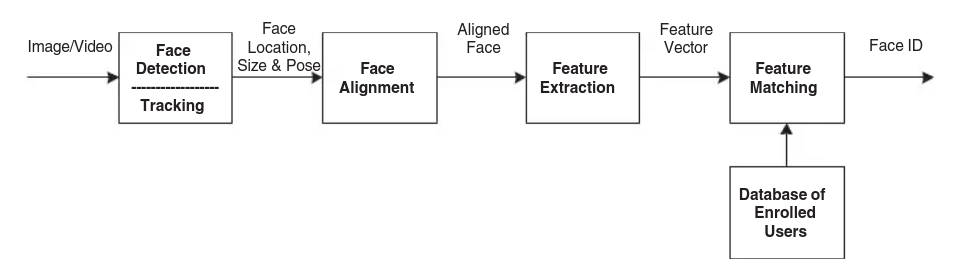
\includegraphics[width=0.8\textwidth]{Cap2_Revisao_Teorica/Figures/fluxo_rec.png}
    \caption*{Fonte: \cite{StanZ.Li2011}}
    \label{fig:fluxoReconhecimento}
\end{figure}

Na etapa de detecção “Face Detection”, temos um vídeo ou uma imagem como entrada. Essa etapa tem como função localizar e extrair uma ou mais faces que estejam presentes na imagem. No caso em que a entrada é um vídeo, se necessário, essa etapa também é responsável pelo rastreamento, “Tracking”, das faces, quadro a quadro. A faces extraídas passam então pela etapa de alinhamento, “Face Alignment”, que é responsável por normalizar a imagem em rotação e em escala, de forma que na imagem resultante a face esteja alinhada ao eixo horizontal do plano. \cite{StanZ.Li2011, Quirita2014}.

Depois de já alinhada, a face passa pela etapa de extração de características, “Feature Extraction”. Essa etapa tem a função de identificar e extrair da face pontos faciais distintos, como olhos, nariz, boca e outras marcas de referência que sejam suficientes para caracterizar a face, de forma que a mesma possa ser distinguida dentre as faces obtidas de outras pessoas. \cite{StanZ.Li2011}. Em seguida são computadas as relações geométricas entre esses pontos faciais, reduzindo-se assim a imagem facial de entrada em um vetor de características geométricas \cite{Jafri2009}. A figura 2.2 destaca alguns pontos faciais característicos e as relações geométricas entre eles.

Os primeiros trabalhos realizados em reconhecimento de faces baseavam-se principalmente nessa técnica. Em uma das primeiras tentativas empregou-se um método simples de processamento de imagem para extrair um vetor de 16 parâmetros faciais, que eram relações de distâncias, áreas e ângulos, de forma a compensar o tamanho variável das imagens. Então usou-se uma medida de distância euclidiana simples para correspondência, chegando a um desempenho máximo de 75\% em um banco de dados de 20 pessoas diferentes, usando 2 imagens por pessoa. \cite{Kanade1977}

\begin{figure}[h]
    \centering
    \caption[Características geométricas (destaque em branco), usada em experimentos de reconhecimento de faces.]{Características geométricas (destaque em branco), usada em experimentos de reconhecimento de faces}
    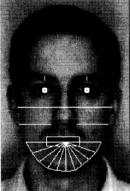
\includegraphics[width=0.2\textwidth]{Cap2_Revisao_Teorica/Figures/face_vetores.png}
    \caption*{Fonte: \cite{StanZ.Li2011}}
    \label{fig:faceVetores}
\end{figure}

Tendo as características geométricas da face calculadas e codificadas em um vetor, a próxima etapa para o reconhecimento da face é fazer a correspondência, ou “Feature Matching” (quarta e última etapa do processo de reconhecimento proposto na figura 1.2). Essa etapa consiste em comparar o vetor obtido da face que se deseja reconhecer com um banco de dados de vetores de outras faces que já são conhecidas e tiveram suas caraterísticas extraídas pelo mesmo processo descrito até aqui. O reconhecimento é feito com base no grau de similaridades entre a face sendo verificada e as faces conhecidas \cite{Quirita2014}.   

A principal vantagem oferecida pelas técnicas de reconhecimento baseadas em características é que, uma vez que a extração dos pontos característicos é anterior à análise feita para comparar a face com a de um indivíduo conhecido, esses métodos são relativamente robustos para variações de posição na imagem de entrada \cite{Jebara1996}. A princípio, esquemas baseados em características podem ser invariáveis ao tamanho, orientação ou iluminação \cite{Cox1996}. Outras vantagens de se utilizar técnicas baseadas em características faciais incluem a compactação de representação das imagens de face e a alta velocidade na tarefa de verificação de correspondência (identificação) \cite{Brunelli1992}.

A principal desvantagem dessa técnica é a dificuldade de detecção automática de características e o fato de que o desenvolvedor da aplicação deve tomar decisões arbitrárias sobre quais características são importantes para o processo de reconhecimento \cite{Cendrillon2000}.

A biblioteca Dlib C++ disponibiliza algumas ferramentas para reconhecimento facial. Em seu site, está disponível gratuitamente um modelo pré-treinado para extração de características faciais, que alcançou uma marca de precisão de 99,38\% no benchmark de reconhecimento facial da \textit{Labeled Faces in the Wild} (LFW) em fevereiro de 2017, que é comparável a outros métodos de última geração para reconhecimento facial. \cite{King2017}. A LFW é uma referência pública para verificação de desempenho de reconhecimento facial \cite{VisionLab2020}.

Esse modelo mapeia a imagem de uma face humana em um vetor de 128 dimensões espaciais. Quando vetores de duas imagens diferentes são muito próximos, significa que a face tende a pertencer à mesma pessoa. Assim, o reconhecimento facial pode ser obtido mapeando-se várias faces em vetores de 128 dimensões e compará-las entre si calculando a distância Euclidiana \cite{Anderson2021}.

Esse modelo foi treinado a partir de um banco de cerca de 3 milhões de imagens. A precisão alcançada de 99,38\% significa que, ao ser apresentada um par de imagens faciais, a ferramenta identificará corretamente se o par pertence à mesma pessoa ou é de pessoas diferentes  em 99,38\% das vezes \cite{King2017}, o que o torna uma boa ferramenta para reconhecimento de faces de uma forma geral.

O grande avanço nas técnicas e ferramentas de aprendizado de máquina abriu um grande leque de possibilidades de aplicações de inteligência artificial nos últimos anos. Devido a isso, os recentes modelos de detecção e reconhecimento, não só de faces, mas de objetos em geral, estão cada vez mais precisos e rápidos. Isso, aliado ao expressivo avanço da Internet das Coisas (IoT), trazendo à tona o conceito de Edge Computing, torna cada vez mais viável as implementações de videomonitoramento automático.


\section{A Internet das Coisas, Edge e Fog Computing}

A Internet das Coisas, ou \textit{Internet of Things} (IoT), é um paradigma de comunicação recente que prevê em um futuro próximo que os objetos da vida cotidiana serão equipados com microcontroladores, transceptores para comunicação digital e pilhas de protocolo adequadas que os tornarão capazes de se comunicarem entre si e com os usuários finais, tornando-se parte integrante da Internet \cite{Atzori2010}.

O conceito de IoT, portanto, visa tornar a Internet ainda mais imersiva e abrangente. Além disso, ao permitir fácil acesso e interação com uma ampla variedade de dispositivos, como, por exemplo, eletrodomésticos, câmeras de vigilância, sensores de monitoramento, atuadores, monitores, veículos e assim por diante, a IoT promoverá o desenvolvimento de uma série de aplicações que fazem uso da quantidade e enorme variedade de dados gerados por tais objetos para fornecer novos serviços aos cidadãos, indústrias e administrações públicas. Esse paradigma encontra aplicação em muitos domínios diferentes, como automação residencial, automação industrial, assistência médica, saúde móvel, assistência a idosos, gerenciamento de energia inteligente e redes inteligentes, automotivo, gerenciamento de tráfego e muitos outros \cite{Bellavista2013}.

Com o advento da Internet das coisas nós estamos em uma era onde haverá uma grande quantidade de dados gerados por coisas que estão imersas em nosso dia a dia. Conforme estimado pela Cisco, em 2019, os dados produzidos por pessoas, máquinas e “coisas” chegaria a 500 zetabytes \cite{Deutscher2015}. Para processar esses todos esses dados, é necessário muito poder computacional.

Hoje em dia, a computação em nuvem é uma plataforma econômica e prevalecente, oferecendo enorme poder de processamento e capacidade de armazenamento para treinamento de modelos de machine learning, reconhecimento facial, reconhecimento de fala, visão computacional, processamento automatizado de linguagem, classificação de texto e diversas aplicações de IoT e smart cities. No entanto, também tem algumas desvantagens importantes, como latência de resposta da rede e a segurança do sistema no que diz respeito a questões de privacidade, já que para chegar na nuvem os dados, possivelmente sensíveis, precisam trafegar por um longo caminho na rede mundial \cite{Pacheco2018}.

A maioria das ações de controle de IoT deve ser realizada em tempo real, portanto, o tempo de espera de processamento em nuvem, principalmente devido à latência da rede, não funciona bem para problemas de IoT \cite{Singh2017}. Na tentativa de contornar algumas dessas limitações, aparecem alguns paradigmas recentes e complementares. São o Fog e o Edge Computing, que promete a capacidade de realizar tarefas de uma forma mais distribuída e responsiva, uma vez que os nós de IoT estão mais próximos das fontes de dados dos sensores. Além disso, também reduz o tráfego de rede e evita a exposição de dados privados do usuário \cite{Pacheco2018}.

A figura \ref{fig:arquitetura} demonstra muito bem a ideia de uma arquitetura de processamento distribuído, indicando as características que cada parte da rede dá à aplicação ao ser responsável por parte do processamento.
\begin{figure}[H]
    \centering
    \caption[Arquitetura de computação distribuída]{Arquitetura de computação distribuída}
    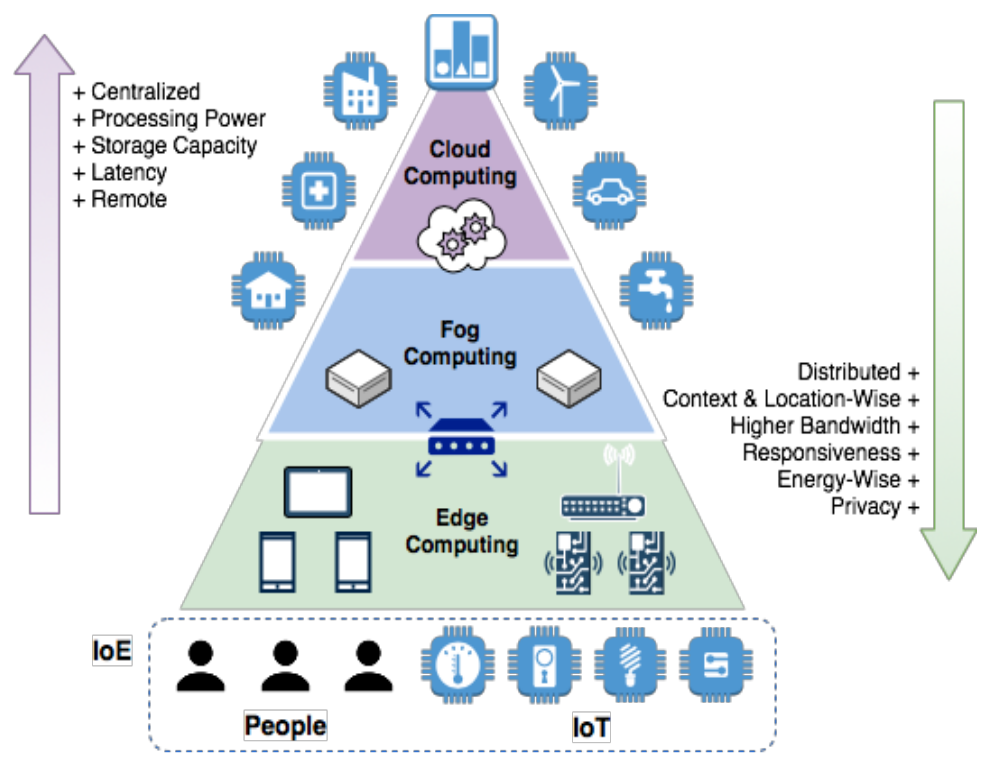
\includegraphics[width=0.9\textwidth]{Cap2_Revisao_Teorica/Figures/arquitetura_distribuida.png}
    \caption*{Fonte: \cite{Pacheco2018}}
    \label{fig:arquitetura}
\end{figure}

